\subsection{Five forces}
 Porter præsenterer også en alternativ måde at forstå et startups succes, kaldet "Five forces".
 Disse ``five forces'' beskriver den konkurrencekontekst som virksomheden indgår i.
 Følgende beskrivelse er baseret på \citet[p.~16]{rose2012software}.

 Ifølge Porter er succesen af et startup delvis defineret af hvordan virksomheden konkurrerer med andre virksomheder på samme marked.
 Porters model kan ses på \cref{fiveforces}.

\begin{figure}[H]
	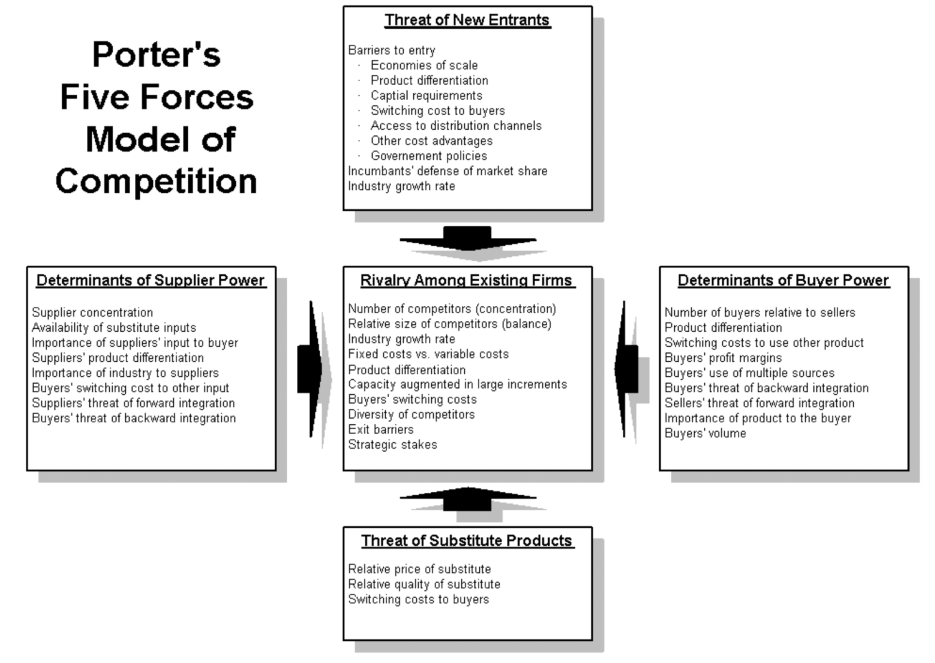
\includegraphics[width=\textwidth]{fiveforces.PNG}
	\caption{Five forces modellen}
	\label{fiveforces}
\end{figure}

\paragraph{Five Forces i SharePass' marked}
\label{par:five_forces_i_sharepass_marked}

For at beskrive det marked SharePass skal konkurrere benyttes Five Forces modellen. 
Hver af de fem markedskræfter er beskrevet med de mest karakteriserende elementer.

\begin{description}
	\item[Rivalry among existing firms] Der findes mange password managers, både ren software og hardware managers. Typisk benyttes en abonnementsmodel.
	\item[Threat of new entrants] Vores produkt har en væsentlig "switching cost"\footnote{Det engelske udtryk ``switching cost'' er brugt i denne kontekst til at beskrive det en kunde skal ændre for at skifte fra et produkt til et andet.}  i forhold til eksisterende løsninger (der dog ikke er lige så integreret i virksomheden). 
	\item [Threat of substitute products] Vores produkt kan få konkurrence af mindre avancerede løsninger der har lavere "switching cost".
	\item [Determinants of Supplier Power] Vores hardware er ikke specifik for en supplier og det er derfor let at skifte. 
	\item [Determinants of Buyer Power] Fokus er at skræddersy til virksomheder hvilket betyder at virksomhederne har en stor magt.
\end{description}
